\documentclass[11pt,a4paper]{article}
\usepackage{polski}
\usepackage[utf8]{inputenc}
\usepackage{listings}
\usepackage{graphicx}
\usepackage{color}
\renewcommand{\floatpagefraction}{0.1}
\title{Dźwięk i muzyka w systemach komputerowych - laboratorium 02}
\author{Marcin Fabrykoski}
\date{}
\begin{document}
\maketitle
\newpage
\begin{enumerate}
\item Naszym zadaniem jest wygenerowanie sygnałów: prostokątnego o~współczynniku wypełnienia 50\% oraz 80\%, piłokształtnego oraz trójkątnego. Obliczenie transformaty Fouriera.\\
Poniżej przedstawiony jest program przykładowy program rysujący sygnał prostokątny o~współczynniku wypełnienia 80\%:
\lstinputlisting[language=Octave,basicstyle=\footnotesize,caption="Zadanie 1"]{zad1.m}
Wyniki widać odpowiednio na rysunkach:
\begin{enumerate}
\item prostokątny, 50\% rys.\ref{fig:pros50}
\item prostokątny, 80\% rys.\ref{fig:pros80}
\item pilokszatłtny rys.\ref{fig:pila}
\item trójkątny rys.\ref{fig:trojkat}
\end{enumerate}
\begin{figure}
\hspace{-10em}
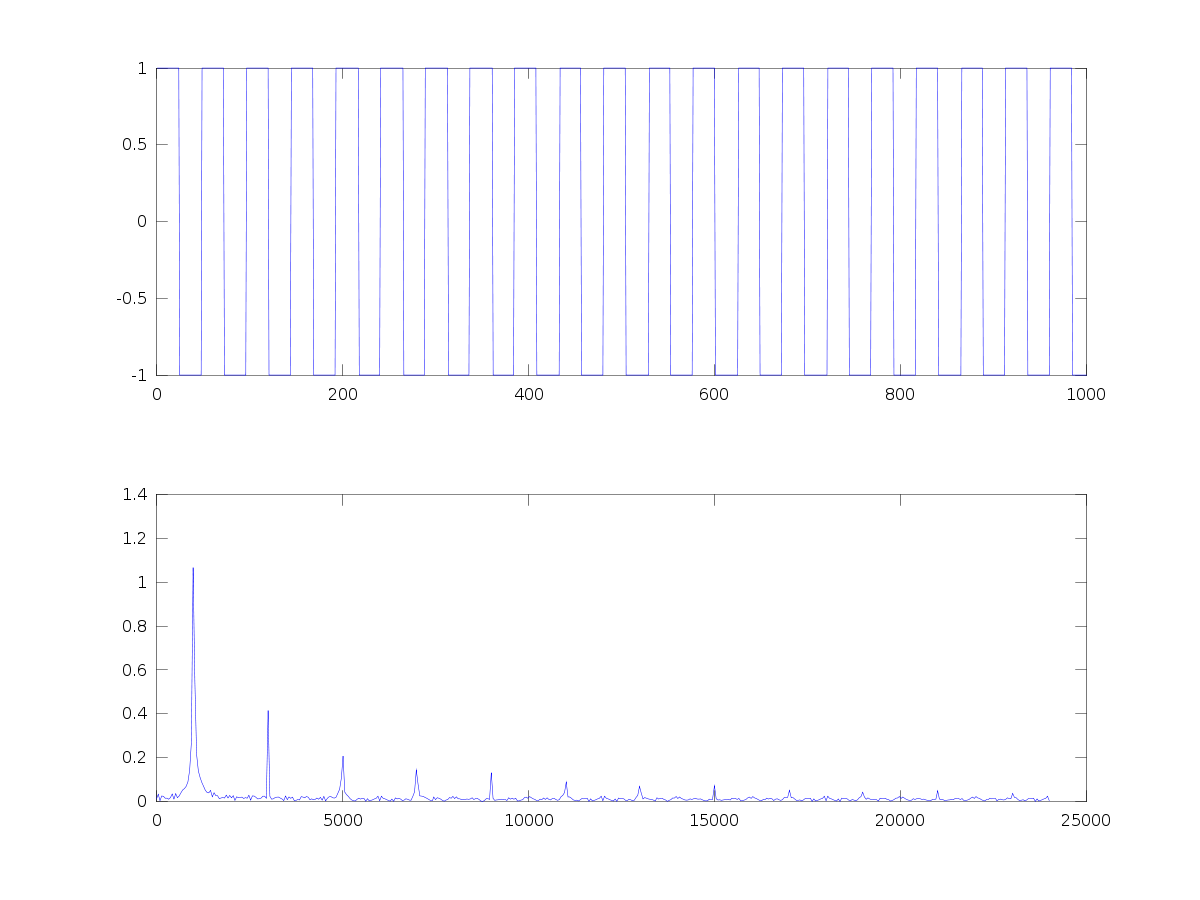
\includegraphics[scale=0.5]{proba1_1.png}
\caption{Prostokątny, 50\%}
\label{fig:pros50}
\end{figure}
\begin{figure}
\hspace{-10em}
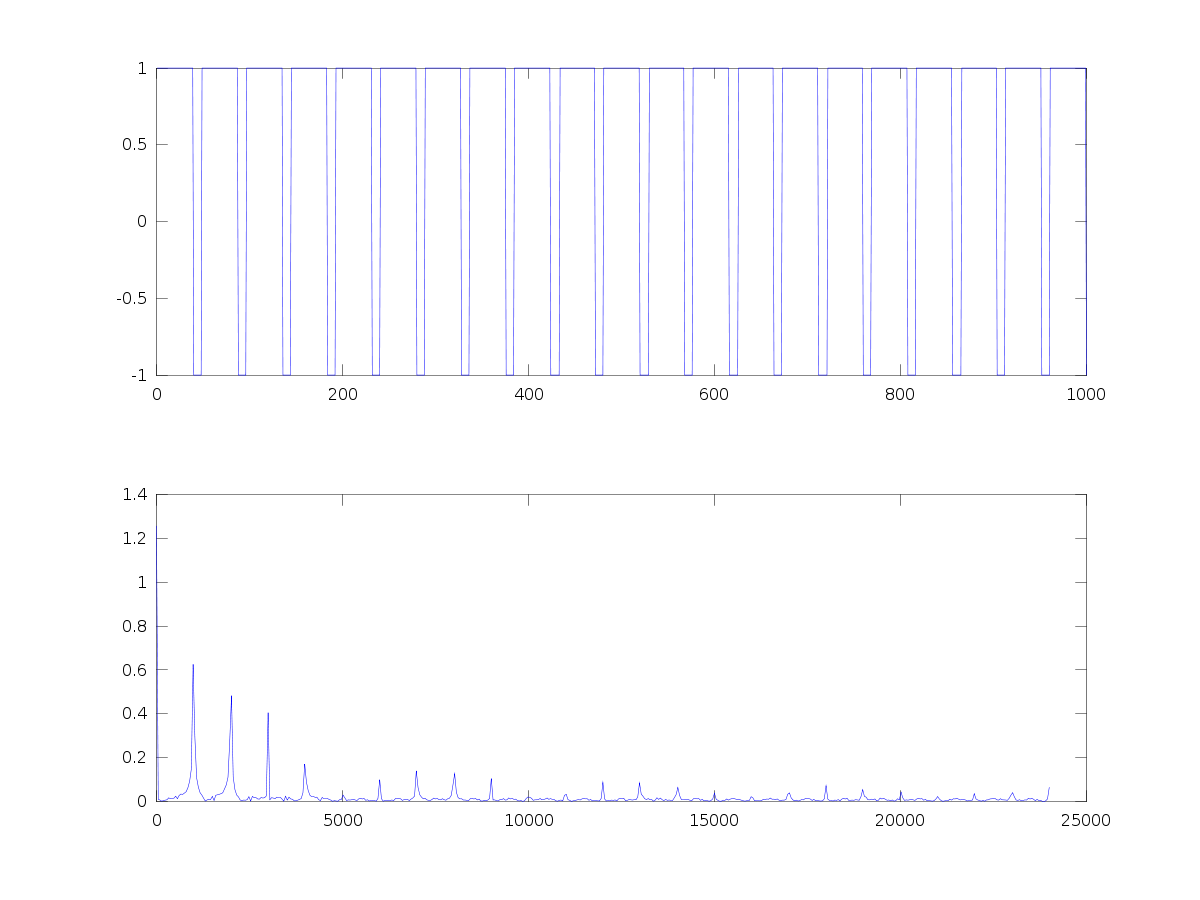
\includegraphics[scale=0.5]{proba1_4.png}
\caption{Prostokątny, 80\%}
\label{fig:pros80}
\end{figure}
\begin{figure}
\hspace{-10em}
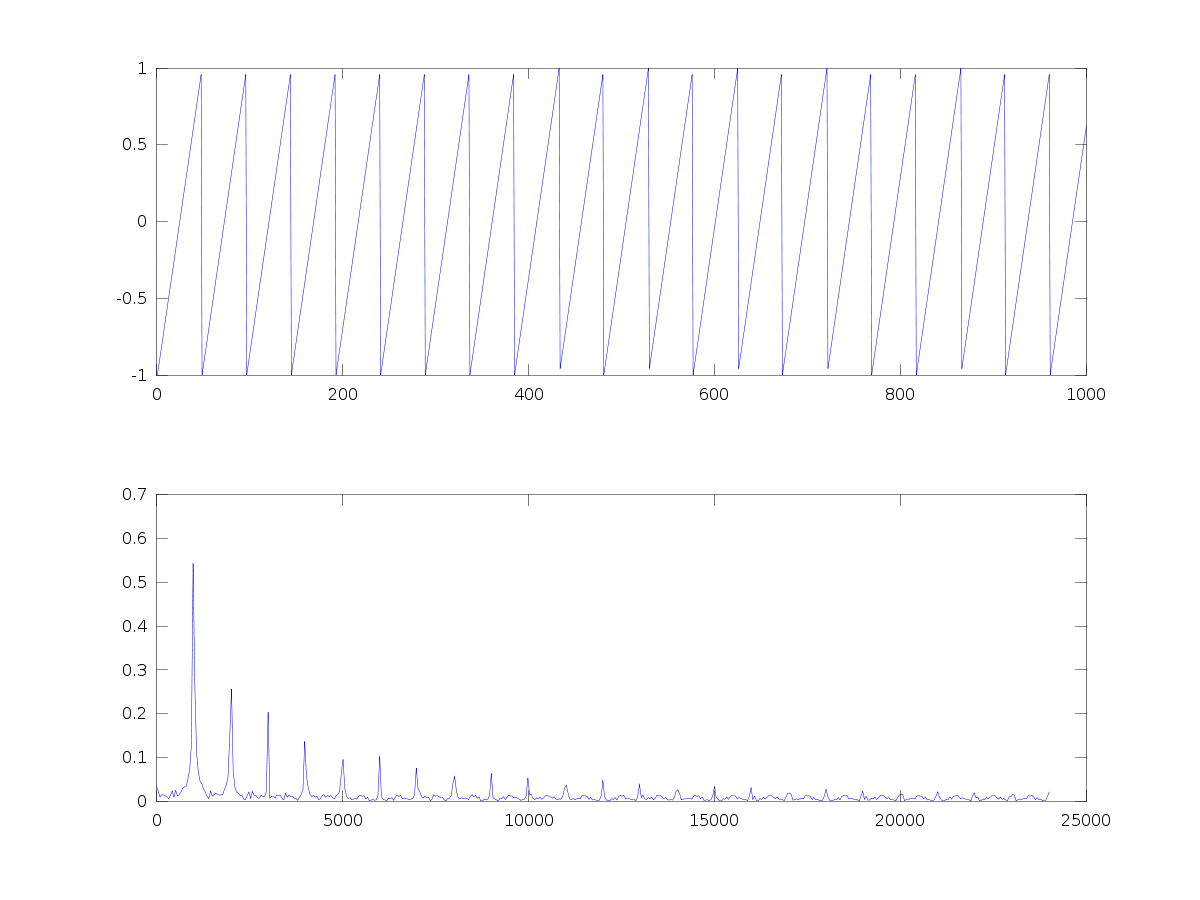
\includegraphics[scale=0.5]{proba1_2.png}
\caption{Piłokształtny}
\label{fig:pila}
\end{figure}
\begin{figure}
\hspace{-10em}
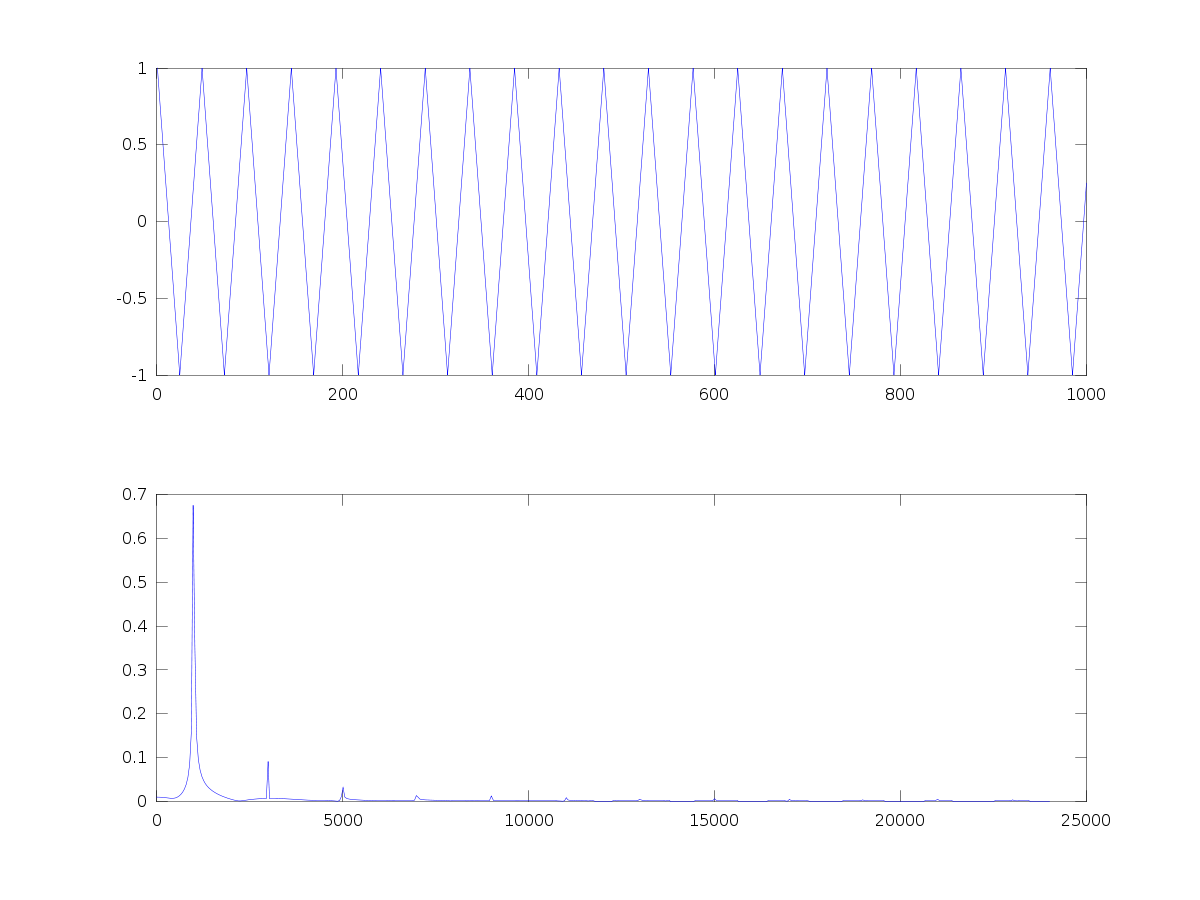
\includegraphics[scale=0.5]{proba1_3.png}
\caption{Trójkątny}
\label{fig:trojkat}
\end{figure}
\newpage
\item Celem tego ćwiczenia jest wygenerowanie sygnału sinusoidalnego o~częstotliwości w~zakresie 50Hz do 5kHz liniowo zmiennego oraz obliczenia jego widma.\\
Zadanie to realizuje poniższy program
\lstinputlisting[language=octave,basicstyle=\footnotesize,caption="Zadanie 2"]{zad2.m}
Czego wynik możemy zaobserwować na rys. \ref{fig:liniowo}
\begin{figure}
\hspace{-10em}
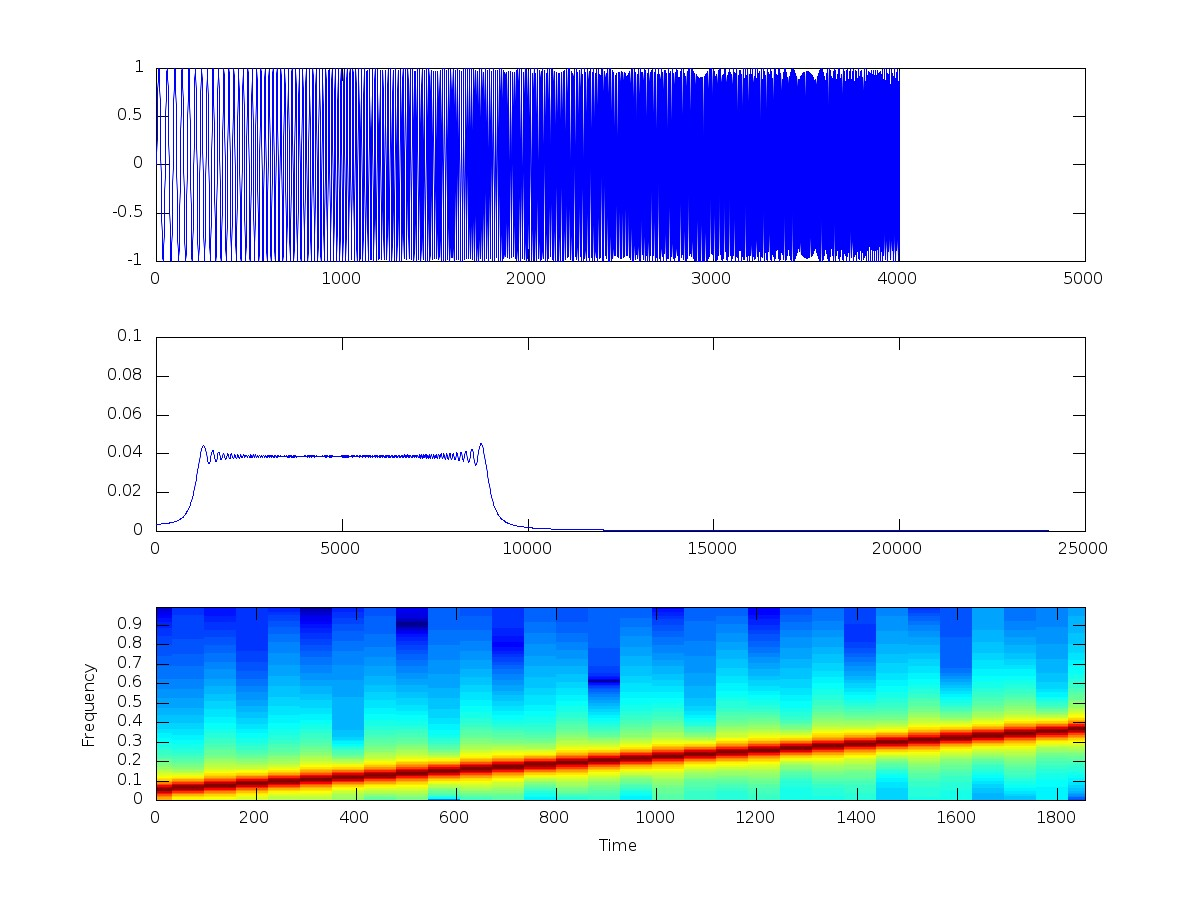
\includegraphics[scale=0.5]{proba2_1.jpg}
\caption{Częstotliwość zmieniana liniowo oraz widmo}
\label{fig:liniowo}
\end{figure}
\newpage
\end{enumerate}
\end{document}
